\documentclass{beamer}

% Romanian Language support
\usepackage{ucs}
\usepackage[utf8x]{inputenc}
\PrerenderUnicode{aâîțșĂÎÂȚȘ}
\usepackage[english,romanian]{babel}

\usepackage{hyperref}   % use \url{http://$URL} or \href{http://$URL}{Name}
\usepackage{verbatim}
\usepackage{underscore} % underscores need not be escaped
\usepackage{booktabs}   % nice looking tables
\usepackage{array}      % column size options in tables
\usepackage[normalem]{ulem}       % for striketrough text

\mode<presentation>
%{ \usetheme{Berlin} }

% Disable useless navigation symbols.
\setbeamertemplate{navigation symbols}{}

\title[Despre dezvăț]{Despre dezvăț: Uneori strici ca să construiești}
\institute{Info Educație 2016 (Gălăciuc, Vrancea)}
\author[Răzvan Deaconescu]{Răzvan Deaconescu \\
razvan.deaconescu@cs.pub.ro}
\date{5 august 2016}

\begin{document}

\frame{\titlepage}

\begin{frame}{În ce direcție merge autobuzul?}
  \begin{figure}
    \centering
    
\includegraphics[width=0.7\textwidth]{img/bus-direction}
  \end{figure}
  \begin{center}
    \scriptsize
    \url{http://www.reatrey.com/wp-content/uploads/2016/02/Screenshot_1-6.jpg}
  \end{center}
\end{frame}

\begin{frame}{Fiz Buzz Test}
  \begin{center}
    \scriptsize
    \url{http://c2.com/cgi/wiki?FizzBuzzTest}
  \end{center}
The Fizz-Buzz test is an interview question designed to help filter out the 99.5\% of programming job candidates who can't seem to program their way out of a wet paper bag. The text of the programming assignment is as follows:

    Write a program that prints the numbers from 1 to 100. But for multiples of three print ``Fizz'' instead of the number and for the multiples of five print ``Buzz''. For numbers which are multiples of both three and five print ``FizzBuzz''.

I think Fizz-Buzz is ``hard'' for some programmers because (\#1) it doesn't fit into any of the patterns that were given to them in school assignments, and (\#2) it isn't possible to directly and simply represent the necessary tests, without duplication, in just about any commonly-used modern programming language.
\end{frame}

\begin{frame}{Experimentul cu maimuțele}
  TODO
\end{frame}

\begin{frame}{It's all about the money}
  \begin{itemize}
    \item Ești manager.
    \item Ai nevoie ca echipa pe care o conduci să vină cu soluții creative la o problemă.
    \item Le spui că le acorzi un bonus de 25\% dacă vin astfel de soluții.
  \end{itemize}
  \begin{center}
    Dan Pink: The Suprising Truth About What Motivates Us\\
    \scriptsize
    \url{http://www.ted.com/talks/dan_pink_on_motivation?language=en}
  \end{center}
\end{frame}

\begin{frame}{Anakin Skywalker}
  citat Yoda
\end{frame}

\begin{frame}{Cum învățăm?}
  de la cei din jur
  din experiență
  din societate
  din ce vedem, auzim, ascultăm
  din ce citim
  de pe Internet
\end{frame}

\begin{frame}{Problema Internet-ului}
  multă informație
  informația nu este filtrată
  îți dă soluția la problemă, nu cum ajungi la ea
  Google/SO considered harmful
  Computers are useless
\end{frame}

\begin{frame}{Imperfecțiuni și inabilități}
  informații incomplete
  obieceiuri ineficiente
  presiune socială: așa e bine, așa se întâmplă
  poveste cu cine nu putea să se strâmbe
\end{frame}

\begin{frame}{De ce se întâmplă?}
  lene
  lipsă de răbdare
  neconștientizarea alternativei
  influență mare a celor din jur
  absența gândirii critice
  bias-uri: confirmation bias
  instinctul de turmă, ,,compliance''
  bulă socială
  experimentul cu maimuțele
  \url{http://www.throwcase.com/2014/12/21/that-five-monkeys-and-a-banana-story-is-rubbish/}
\end{frame}

\begin{frame}{De ce e rău că se întâmplă?}
  împrăștii dezinformare, cultivare de ignoranță
  nu îți atingi potențialul, te auto-limitezi
  te rigidizezi, nu te adaptezi, fosilizare
  lumea este în mișcare rapidă, e dinamică
\end{frame}

\begin{frame}{Cea mai bună întrebare. Cel mai bun răspuns.}
  stai în banca ta
  bagă-te în față, dă din coate
  Winston Churchill
\end{frame}

\begin{frame}{Despre dezvăț}
  renunțat la obiceiuri, comportamente, gânduri, moduri de abordare
  alterat obiceiuri, comportamente, gânduri, moduri de abordare
  stricat și construit
  Pink Floyd: Another Brick in the Wall
\end{frame}

\begin{frame}{Exemple și discuție}
  Răzvan
\end{frame}

\begin{frame}{Pași}
  conștientizare
  găsit soluție
  efort
  reconstruire
  menținut flexibilitate
\end{frame}

\begin{frame}{Cum conștientizăm?}
  introspecție
  ,,citim'' în jur
  \begin{figure}
    \centering
    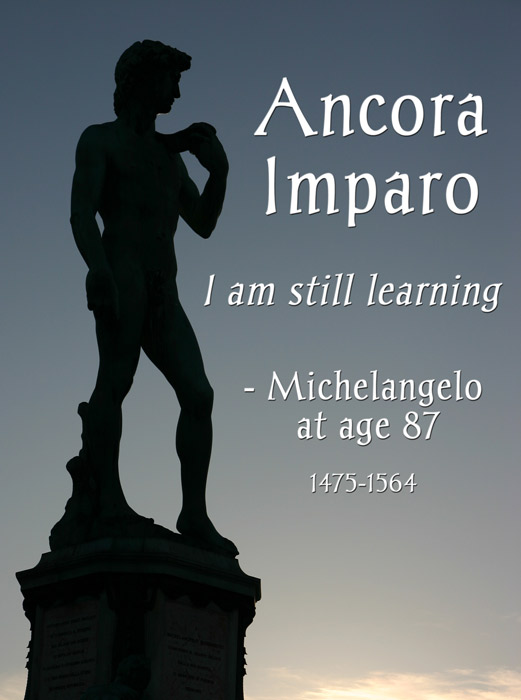
\includegraphics[width=0.4\textwidth]{img/michelangelo-ancora-imparo.jpg}
  \end{figure}
  \begin{center}
    \scriptsize
    \url{https://lh4.ggpht.com/-rCK887WJWO4/V6H7zXtJpJI/AAAAAAB57U0/9THgZkHaQ5c/w560/socialfeed-true-friendship-is-about-tough-love-9gag-mobile-app-www9gagcommobileref9fbp.jpg}
  \end{center}
  Primirea feedback-ului: Denial, Anger, Withdrawal, Acceptance
  oferă, primește, cere, folosește, ia-o de la capăt
\end{frame}

\begin{frame}{Cum construim?}
  acceptarea imperfecțiunilor
  puterea de a spune nu știu
  puterea de a nu te băga în ce nu ține de tine
  conservarea timpului, atenției și energiei
  filtarea exteriorului
  \textit{
  Nu vorbi fără să știi \\
  Nu hali mereu ce auzi de la alții, \\
  Nu te da ce nu poți să fii \\
  Sunt vorbe de c***t, le-aud în fiecare zi \\
  }
  La Familia feat. Uzzi: Vorbe
\end{frame}

\begin{frame}{Recomandări}
  Gândiți-vă la probleme, nu doar la soluții.
  Faceți jocuri de logică, gândire laterală.
  Călătoriți și stați printre oameni.
  Interacționați cu oameni diferiți.
  Jocuri de logică și gândire laterală.
  Faceți puzzle-uri (Enigma: \url{https://www.puzzlemaster.ca/browse/wire/308-cast-enigma-metal})
  \textit{My mind is my weapon. My brother has his sword, King Robert has his warhammer and I have my mind\ldots{} and a mind needs books as a sword needs a whetstone if it is to keep its edge. That's why I read so much, Jon Snow.}\\
  Tyrion Lannister
\end{frame}

\begin{frame}{Recomandări (2)}
  Folosiți mai multe limbaje de programare. Contează problema nu limbajul.
  Învățați programare funcțională.
  Folosiți Linux.
  Faceți lucrurile și altfel.
\end{frame}

\begin{frame}{Recomandări (3)}
  Meditați, analizați-vă.
  Explorați-vă.
  Cereți feedback. Acceptați feedback.
  Enjoy!
\end{frame}

\begin{frame}{În loc de final}
  \begin{figure}
    \centering
    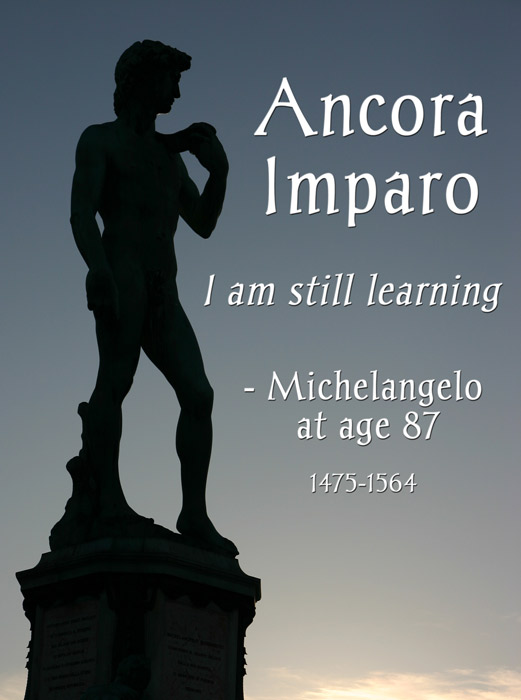
\includegraphics[width=0.4\textwidth]{img/michelangelo-ancora-imparo.jpg}
  \end{figure}
  \begin{center}
    \scriptsize
    \url{http://learnteachserve.org/wp-content/uploads/2014/04/michelangelo_ancora-imparo.jpg}
  \end{center}
\end{frame}

\end{document}
